%%%%%%%%%%%%%%%%%%%%%%%%%%%%%%%%%%%%%%%%%%%%%%%%%%%%%%%%%%%%%%%%%%%%%%%%
% Preamble
%%%%%%%%%%%%%%%%%%%%%%%%%%%%%%%%%%%%%%%%%%%%%%%%%%%%%%%%%%%%%%%%%%%%%%%%
\documentclass[11pt]{article}
%
% Packages and other includes
% Pagination
\usepackage[letterpaper, margin=1.25in]{geometry}
%
% Fonts
\usepackage[T1]{fontenc} % best for Western European languages
\usepackage{lmodern} % Latin Modern instead of CM
\usepackage{textcomp} % required to get special symbols
%
% Math
\usepackage{amsmath, amssymb}
\usepackage{braket}
%
% Graphics, floats, tables
\usepackage{graphicx, xcolor, float, array}
%
% Hyperlinks
\usepackage{hyperref}
%
% Bibliography
\usepackage[style=numeric, sorting=none, backend=biber]{biblatex}
\addbibresource{references.bib}
%
% Revision (see Makefile)
%\input{revision.tex}
%
% Definitions and settings
% Paragraph indent and spacing
\setlength{\parskip}{0.4\baselineskip}
\setlength{\parindent}{0in}
%
% Math mode version of "r" column type (requires array package)
\newcolumntype{R}{>{$}r<{$}}
%
%comments
\newcommand{\brian}[1]{{\color{orange} #1}}
% Title, authors, date
\title{\textbf{Is TPSS an TPSSh better for TPAA calculations?}}
\author{Thanh Huynh and Brian Nguyen}
\date{11/27/2020 -- 01/10/2021 }
%
%
%%%%%%%%%%%%%%%%%%%%%%%%%%%%%%%%%%%%%%%%%%%%%%%%%%%%%%%%%%%%%%%%%%%%%%%%
% Main document
%%%%%%%%%%%%%%%%%%%%%%%%%%%%%%%%%%%%%%%%%%%%%%%%%%%%%%%%%%%%%%%%%%%%%%%%
%

\begin{document}

\maketitle

\section{Introduction}

\brian{Mention big picture -> lissoclimide project; follow-up to the
  previous report}
The TPSS and TPSSh functionals may describe the halogen-pi bond more
accurately than PBE. To investigate which functional performs better,
the X40 test set serves as a benchmark for TPSS, TPSSh, and PBE 
calculations.  


\section{Methods}

\brian{Most of calculations are based on the previous report. The 3-4
  extrapolation of the RIRPA correlation energy was good balance between
  efficiency and accuracy...}
The X40 Test Set was used the benchmark the method's accuracy for 
noncovalent interactions involving halogens \brian{remind your reader
  of the x40 test set - descriptions: type of interactions, and how
  many complexes}. Calculations were computed
with basis sets def2-QZVP, cc-pVTZ, and cc-pVQZ. The RPA energies were
computed based on converged orbitals from TPSS and TPSSh and resolution
of identity (RI) was included to improve efficiency. 

\brian{For the sake of time,} a set of eight complexes from X40 test set
was chosen to study basis set convergences based on error from a previous
report. 

\section{Results}

\brian{Adding figures - lookup how to add figures; see Fig. \ref{fig:rpa_basis}
  as good example}

\begin{figure}[hbpt]
  \centering
  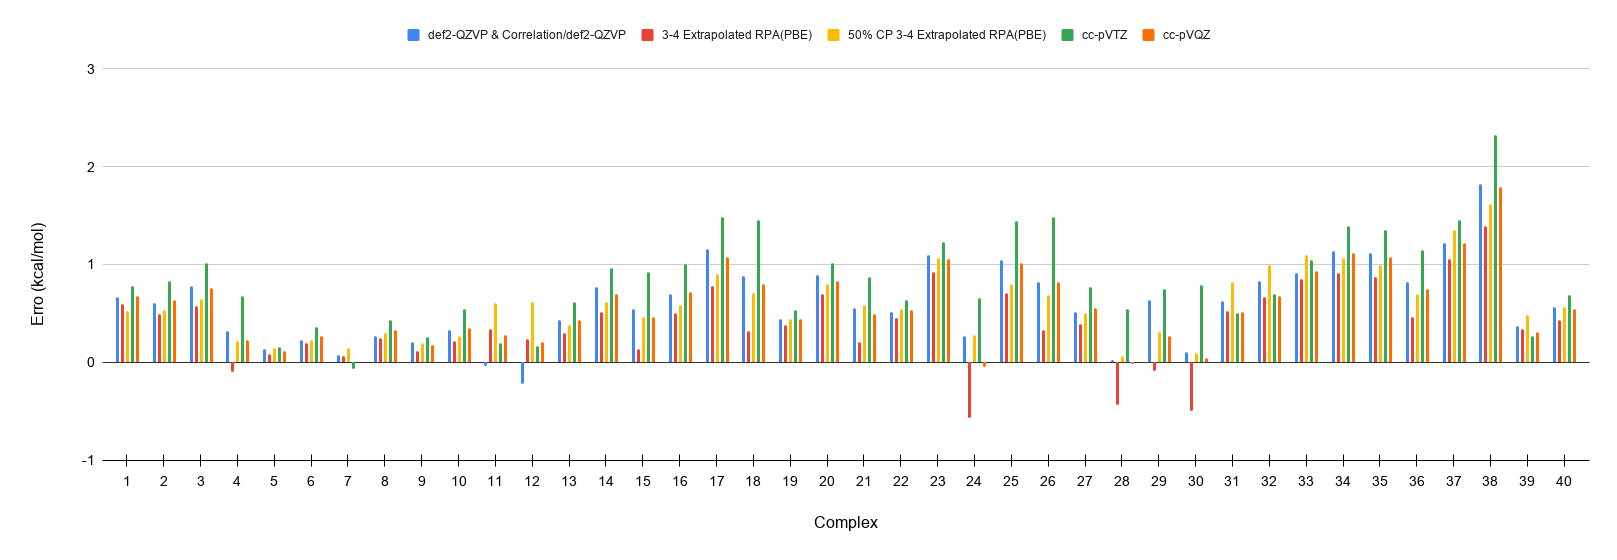
\includegraphics[scale=0.25]{def2-QZVP_error.png}
  \caption{The binding energy errors (kcal/mol) for X40 test set computed
    for PBE, PBE-D3, PBE-D4, RPA(PBE), and def2-QZVP. All methods were 50
    CP corrected and negative sign indicates overbinding.}
  \label{fig:rpa_basis}
\end{figure}

\begin{figure}[hbpt]
  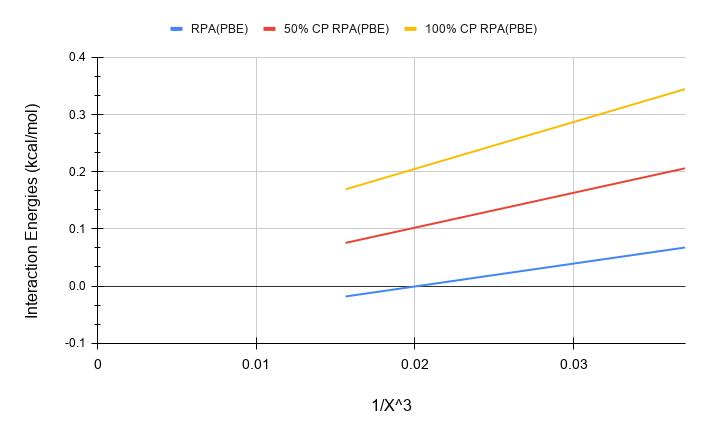
\includegraphics[scale=0.5]{tpss_1.png}
  \caption{This is a figure.}
  \label{fig:<name>}
\end{figure}

\begin{figure}
  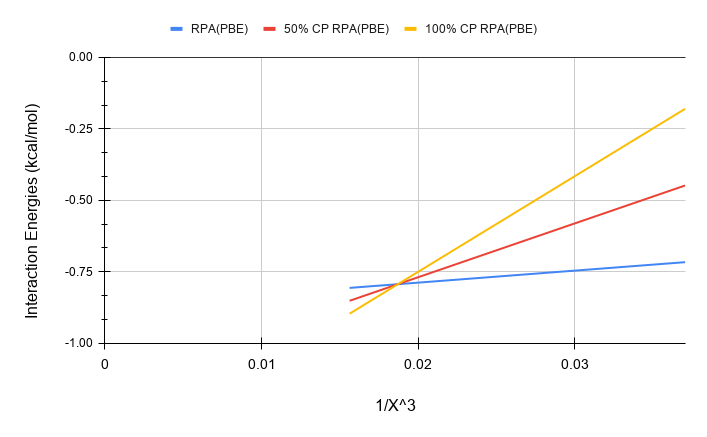
\includegraphics[scale=0.5]{tpss_8.png}
  \caption{This is a figure.}
  \label{fig:<name>}
\end{figure}

\begin{figure}
  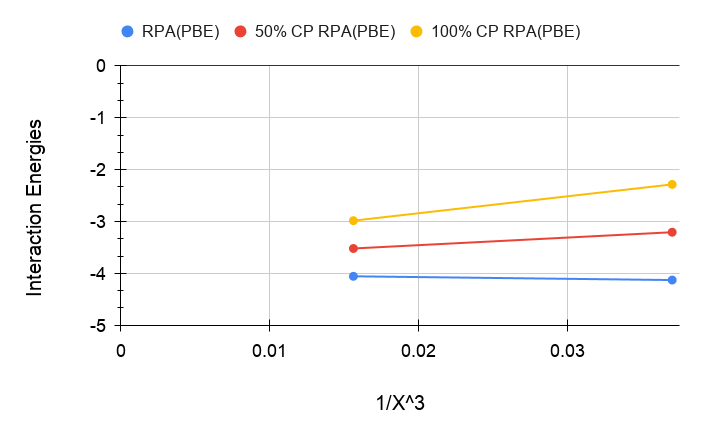
\includegraphics[scale=0.5]{tpss_11.png}
  \caption{This is a figure.}
  \label{fig:<name>}
\end{figure}

\begin{figure}
  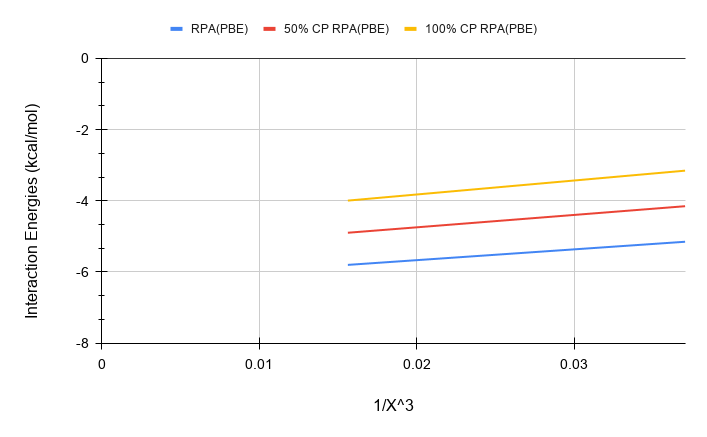
\includegraphics[scale=0.5]{tpss_24.png}
  \caption{This is a figure.}
  \label{fig:<name>}
\end{figure}

\begin{figure}
  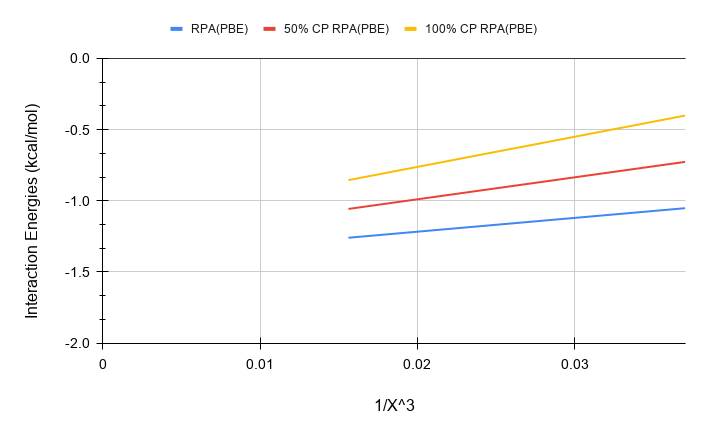
\includegraphics[scale=0.5]{tpss_27.png}
  \caption{This is a figure.}
  \label{fig:<name>}
\end{figure}

\begin{figure}
  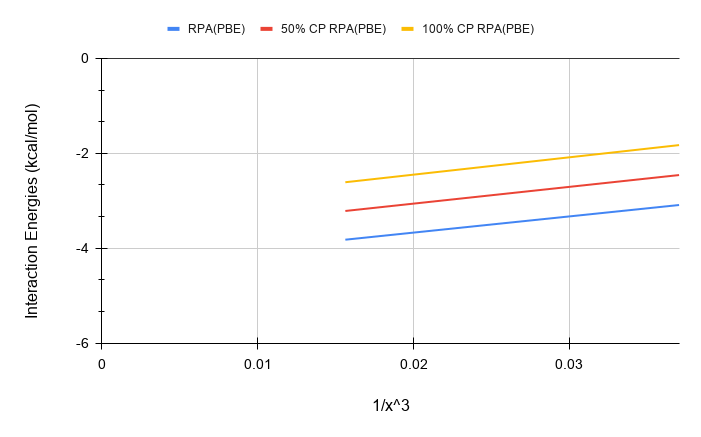
\includegraphics[scale=0.5]{tpss_30.png}
  \caption{This is a figure.}
  \label{fig:<name>}
\end{figure}

\begin{figure}
  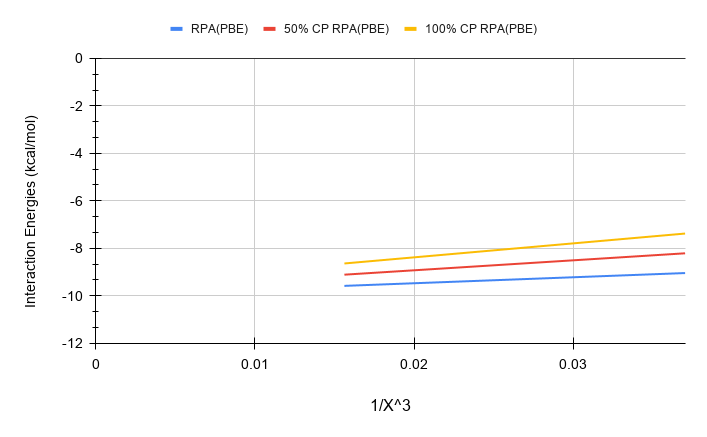
\includegraphics[scale=0.5]{tpss_38.png}
  \caption{This is a figure.}
  \label{fig:<name>}
\end{figure}

\begin{figure}
  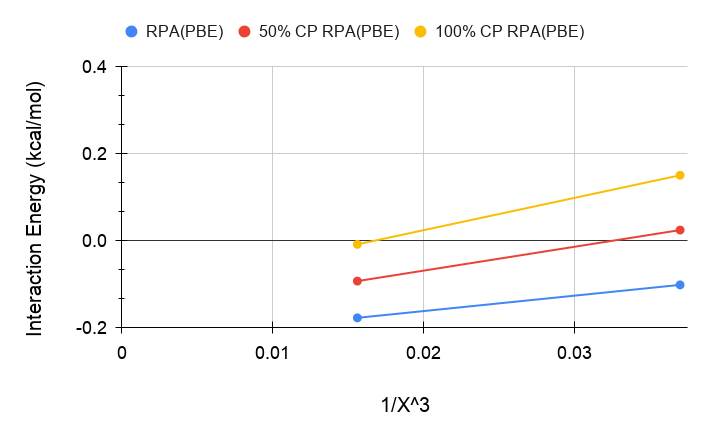
\includegraphics[scale=0.5]{tpssh_1.png}
  \caption{This is a figure.}
  \label{fig:<name>}
\end{figure}

\begin{figure}
  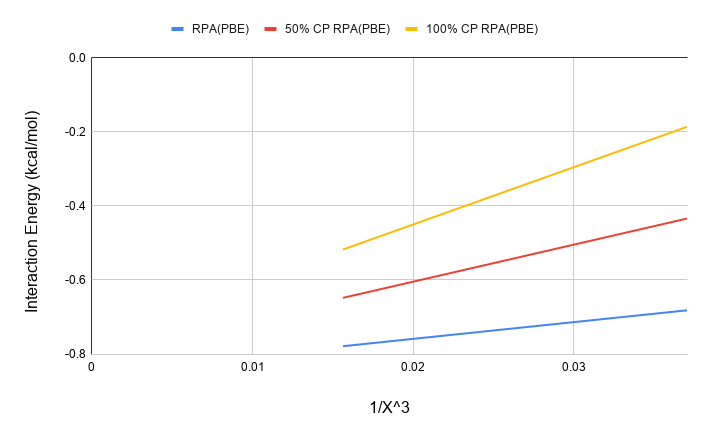
\includegraphics[scale=0.5]{tpssh_8.png}
  \caption{This is a figure.}
  \label{fig:<name>}
\end{figure}

\begin{figure}
  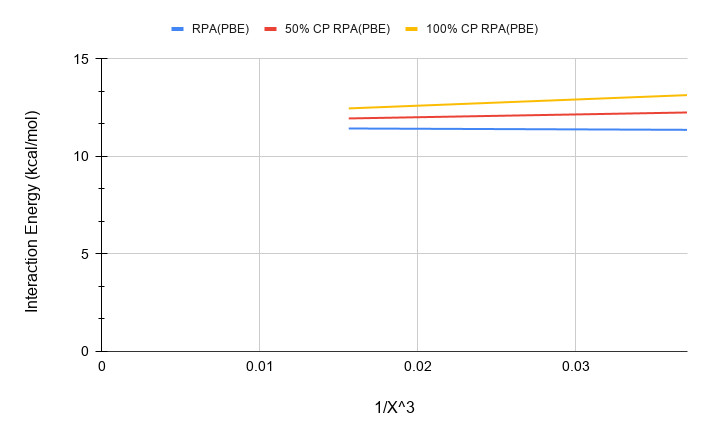
\includegraphics[scale=0.5]{tpssh_11.png}
  \caption{This is a figure.}
  \label{fig:<name>}
\end{figure}

\begin{figure}
  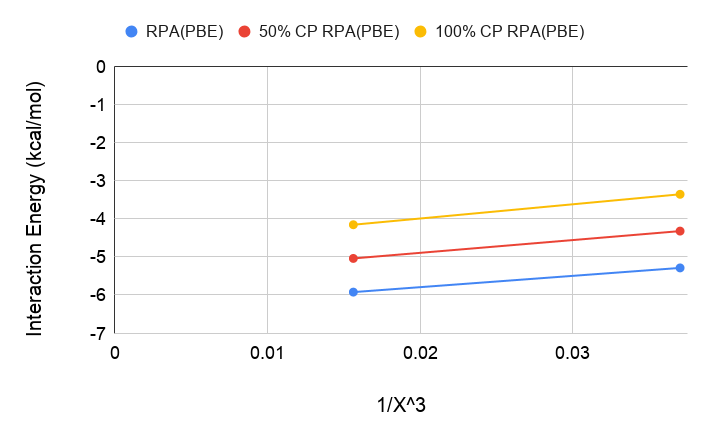
\includegraphics[scale=0.5]{tpssh_24.png}
  \caption{This is a figure.}
  \label{fig:<name>}
\end{figure}

\begin{figure}
  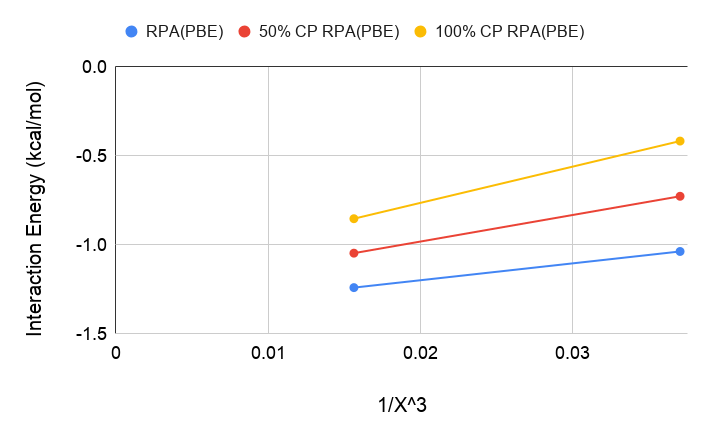
\includegraphics[scale=0.5]{tpssh_27.png}
  \caption{This is a figure.}
  \label{fig:<name>}
\end{figure}

\begin{figure}
  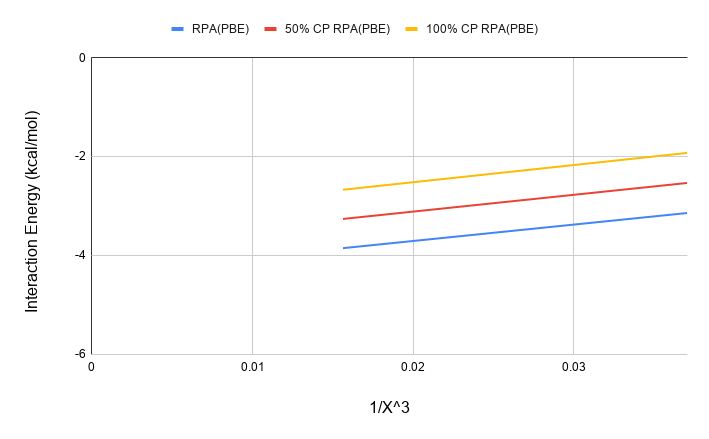
\includegraphics[scale=0.5]{tpssh_30.png}
  \caption{This is a figure.}
  \label{fig:<name>}
\end{figure}

\begin{figure}
  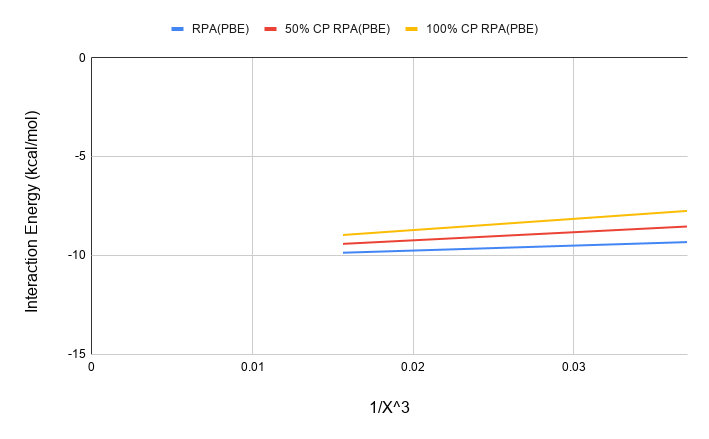
\includegraphics[scale=0.5]{tpssh_38.png}
  \caption{This is a figure.}
  \label{fig:<name>}
\end{figure}


\brian{yada yada see Fig. \ref{fig:<name>}}
This section states the main new results of the current
reporting period. These results could be presented, e.g., in the form of
equations, figures, tables, and text. Negative results are just as
important as positive ones and should be carefully reported. Use a
balanced tone avoiding over- and understatement. 

Sometimes, it is helpful to separate statement of the results and
discussion, although a strict separation of the two is often
impossible. A separate discussion section may be appropriate if you are
proposing a speculative rationale or if several interpretations of your
results are possible. If you have no new results at all, this is the
place to explain why. 

\section{Conclusions}


This section should answer the following questions:
What is the significance of your results for the question, problem, or
hypothesis posed in the introduction? What, if any, are the
implications in the broader context of the research area laid out in the
second paragraph of the introduction? 

A second paragraph should discuss any conclusions for your future work. 
Is there a need to change your approach or your priorities? What remains
to be done to reach the goals stated in the first section? 

\printbibliography

\end{document}
